\documentclass[11pt,letterpaper]{article}
\usepackage[margin=1in]{geometry}
\usepackage[T1]{fontenc}
\usepackage{lmodern,microtype}
\usepackage{amsmath,amssymb,amsthm,mathtools}
\usepackage{booktabs,graphicx,array,longtable,placeins}
\usepackage[round,authoryear]{natbib}
\usepackage{xcolor,xurl}
\usepackage[colorlinks=true,linkcolor=blue!40!black,citecolor=blue!40!black,urlcolor=blue!40!black]{hyperref}
\graphicspath{{figures/}}
\newtheorem{proposition}{Proposition}
\newtheorem{corollary}[proposition]{Corollary}
\newtheorem{example}[proposition]{Example}
\newcommand{\E}{\mathbb E}
\newcommand{\Var}{\operatorname{Var}}
\newcommand{\Cov}{\operatorname{Cov}}
\newcommand{\R}{\mathbb R}
\newcommand{\ind}{\mathbf 1}
\newcommand{\argmin}{\operatorname*{arg\,min}}
\newcommand{\argmax}{\operatorname*{arg\,max}}
\newcommand{\MSE}{\operatorname{MSE}}
\setlength{\parskip}{3pt}
\setlength{\emergencystretch}{2em}
\clubpenalty=10000
\widowpenalty=10000
\newcommand{\RawHrmse}{0.1296}
\newcommand{\RawVrmse}{0.1301}
\newcommand{\MeanVrmse}{0.1274}
\newcommand{\CovVrmse}{0.1291}
\newcommand{\SelectedChange}{-0.0245}
\newcommand{\SelectedDecline}{0.0245}
\newcommand{\PeerChange}{-0.0635}
\newcommand{\AdjustedChange}{0.0391}

\title{Before You Target: Ranking Sensitivity and Regression to the Mean in NHS Staff Wellbeing Data}
\author{Shengwei Zhang\\University of Pennsylvania}
\date{September 11, 2026}
\hypersetup{pdfauthor={Shengwei Zhang},pdftitle={Before You Target: Ranking Sensitivity and Regression to the Mean in NHS Staff Wellbeing Data}}

\begin{document}
\maketitle
\begin{abstract}
Selecting the lowest-scoring units for staff wellbeing support creates a decision problem that is easily confused with an intervention evaluation. We distinguish latent severity, membership of the true lowest-scoring set, future observed scores, and intervention benefit. Using established Gaussian and decision-theoretic tools, we derive a conditional decomposition of selected-group change, an exact risk criterion for fixed temporal pooling, and pairwise noise thresholds that determine when a working shrinkage ranking changes. An observational-equivalence construction shows why successful score prediction alone cannot identify latent reliability or, under heterogeneous latent variance, latent rankings. We then analyse official NHS Staff Survey burnout sub-scores for 2021--2025: 190 complete-history reporting units, representing 189 known legal entities. A retrospective backtest uses archived 2023 and 2024 predictor vintages, alongside a separate 2025-reweighted historical panel. Development-selected mean reversion yields a 2025 RMSE of \MeanVrmse{}, compared with \RawVrmse{} for the latest score; the paired entity-bootstrap interval for the improvement includes zero. The 2024 lowest-scoring group declines by \SelectedDecline{} points in 2025 despite improving relative to its benchmark groups. Within a declared static noise-ratio range, 34 of 36 selected units remain selected throughout, indicating limited ranking changes in this particular organisation-level cohort. Six hundred thousand independent Gaussian panel simulations separate latent ranking performance from model-implied rebound and demonstrate failures under misspecification. The results support assumption-sensitive review prioritisation; they do not identify untreated counterfactuals, departmental reliability cutoffs, or optimal health-budget allocations.
\end{abstract}

\section{Introduction}
An employee survey can identify units whose staff report unusually difficult working conditions. A manager deciding where to investigate first may therefore prioritise the units with the lowest scores. Two questions immediately follow. How much of an extreme score reflects persistent need rather than measurement variation? If the selected units improve in the next survey, how much improvement would have occurred without the subsequent action? These questions are connected by selection, but the available data do not necessarily identify either answer.

Consider an illustrative worst-first rule: within each comparable organisation type, reserve a fixed number of review places for the lowest observed burnout sub-scores. This is a policy to analyse, not an assertion that all NHS organisations allocate wellbeing budgets this way. Lower sub-scores indicate less favourable staff experience. Ranking such scores can serve as a screening device, but the units with the greatest underlying difficulty need not have the greatest marginal benefit from a particular intervention. An optimal spending decision would additionally require costs, intervention effects, staff coverage and an explicit equity objective.

Uncertainty in institutional league tables is well established \citep{goldstein1996league}. So are regression to the mean after selecting extreme measurements \citep{barnett2005rtm}, empirical Bayes monitoring of healthcare providers \citep{houwelingen2020monitoring}, and loss-specific ranking under heterogeneous precision \citep{lin2006ranking,gu2023invidious}. The remaining practical problem addressed here is interpretive and empirical: a familiar statistical adjustment can be placed in a decision workflow while making claims that its inputs cannot support. A respondent count is not automatically an effective sample size; a forecast residual is not automatically an intervention effect; and good prediction of a later observed score does not establish recovery of a current latent rank.

We examine these distinctions in the English NHS Staff Survey. Its public organisation-level results permit a substantial reproducible panel analysis, while their limitations are unusually relevant to the decision. The survey reports repeated organisation means rather than a linked individual panel, the organisation scores are occupation-weighted, and historical values can be revised and reweighted in later releases. The published files do not supply the individual weights and composite-score covariance needed to calculate design-based standard errors from scratch. They also contain no identified untreated group or recorded allocation of wellbeing budgets.

The evidence produces a restrained answer. In a five-year complete-history cohort, more complicated temporal rules have small or negative improvements over the latest score when forecasting 2025. A static sensitivity analysis changes only a small part of a within-benchmark review list over a wide declared range of a working variance ratio. Nevertheless, neither stability nor prediction identifies latent need. The selected 2024 low-score group actually declines in 2025, illustrating how a common deterioration can outweigh an improvement relative to peers. Calling every subsequent increase an intervention effect, or promising an increase merely because a unit was selected, would be unjustified.

Our contribution has three parts. First, we assemble exact identities and counterexamples around a common decision, making their assumptions and distinct loss functions explicit. The affine pair-crossing calculation provides a transparent restricted sensitivity diagnostic. Second, we execute a version-aware NHS analysis, separating a harmonised historical holdout from a backtest that uses archived predictor releases available before the target survey waves. Third, paired latent-truth simulations quantify the difference between estimating severity, recovering set membership, and predicting selection-induced change. The value lies in the linked diagnosis and audited application; we do not propose a new general empirical Bayes estimator or claim that regression to the mean is a new phenomenon.

\section{Related work and the decision being studied}
\paragraph{Institutional comparison and provider monitoring.}
\citet{goldstein1996league} describe the statistical and contextual limitations of institutional performance tables. \citet{houwelingen2020monitoring} directly study repeated healthcare-provider comparisons with Gaussian empirical Bayes prediction, autoregressive latent structures and size-related precision. This is a close predecessor to the temporal working model used here. \citet{xia2022profiling} address variation beyond provider control and robustness across provider sizes. These studies caution against equating all between-unit dispersion with management quality or all size-related dispersion with sampling variance.

\paragraph{Ranking depends on the loss.}
\citet{lin2006ranking} develop rankings under different losses, including classification relative to percentile cutpoints. \citet{henderson2016cut} study agreement between selected lists while accounting for unequal precision. \citet{gu2023invidious} formulate ranking and selection as compound decisions with heterogeneous measurement precision; \citet{gang2026ranking} study constrained selection of heteroscedastic units. Our distinction between expected selected severity and true-bottom-set overlap is an application of these established decision principles. It does not imply that either criterion is universally preferable.

\paragraph{Robustness and verification.}
\citet{henderson2025robust} target empirical Bayes estimation to ranking loss under regression-model misspecification. Our one-dimensional noise-ratio analysis is more restricted: it holds the centring and latent-variance structure fixed and identifies algebraic ranking changes as one common multiplier varies. It is also distinct from frequentist verification of Gaussian ranks with specified standard errors \citep{goldwasser2025verification}. A deterministic statement about a working-model parameter interval is not a probability guarantee that the selected NHS units are truly the worst.

\paragraph{Selective follow-up.}
\citet{barnett2005rtm} explain why selecting extreme initial measurements produces apparent subsequent changes. We give a conditional autoregressive decomposition that separates common trends, latent mean reversion and measurement reversion. This decomposition is useful for interpreting an evaluation design, but identifying a no-intervention counterfactual requires additional information. Standard Gaussian conditioning and filtering underlie the calculations \citep{kalman1960filter}.

\paragraph{Scope of the action.}
Let $S$ be a set of $k$ units selected for additional review, with equal per-unit capacity cost. The units can be organisations or, in a hypothetical simulation, smaller administrative units. We evaluate this capacity-constrained review rule. Neither the mathematical action nor the public NHS data specifies a monetary budget, an intervention, the number of staff who would benefit, or the causal effect of spending. We use the term \emph{prioritisation} with that restricted meaning throughout.

\section{Measurements, latent targets and identification}
\subsection{A reference model}
Work within one benchmark group. Let $Y_{it}$ denote the observed score of unit $i$ in year $t$, with a larger value representing better staff experience. Write
\begin{equation}
 Y_{it}=\mu_t+X_{it}+e_{it},\qquad
 X_{i,t+1}=\phi X_{it}+\eta_{i,t+1},
 \label{eq:model}
\end{equation}
where $X$ is initially stationary Gaussian with variance $\tau^2$, $|\phi|<1$, and $\eta_{i,t+1}\sim N\{0,\tau^2(1-\phi^2)\}$. The baseline reference model has independent Gaussian measurement errors $e_{it}\sim N(0,R_{it})$, independent of $X$ and of other units. The common mean path $\mu_t$ is treated as known in the exact identities. Empirical plug-in centring and dependent errors are addressed separately.

Define $\theta_{it}=\mu_t+X_{it}$. This latent target is a mean under a specified survey and standardisation scheme; it is not a clinical diagnosis or a direct measure of management quality. Current $\theta_{it}$, future $\theta_{i,t+1}$ and future observed $Y_{i,t+1}$ are different estimands. Public next-year tables directly validate only the last of these.

The frequently used restriction $R_{it}=\sigma^2/n_{it}$ requires more than an available count. In weighted survey data, $n_{it}$ may be a nominal valid-response count rather than an effective sample size, while the individual composite variance and response-selection process remain unknown. We therefore treat inverse-count precision as a working specification, and vary its scale rather than claiming that the public table identifies it.

\subsection{What aggregate observations can identify}
The identity
\begin{equation}
 \Var(Y\mid n)=\Var(\theta\mid n)+\Var(e\mid n)
                  +2\Cov(\theta,e\mid n)
 \label{eq:variance_size}
\end{equation}
reduces to $\tau^2+\sigma^2/n$ only if the latent variance is constant with size, the measurement variance has the stipulated inverse-count form, and the conditional covariance vanishes. Differences in organisation type, staffing and response selection can violate these assumptions. A positive intercept or a satisfactory regression fit does not independently establish them.

Repeated measurements can identify a decomposition under sufficiently strong restrictions. For a stationary common AR(1) latent process with white, homoscedastic measurement noise and nonzero lag covariances $\gamma_1,\gamma_2$, population moments imply
\begin{equation}
 \phi=\frac{\gamma_2}{\gamma_1},\qquad
 \tau^2=\frac{\gamma_1^2}{\gamma_2},\qquad
 R=\gamma_0-\frac{\gamma_1^2}{\gamma_2}.
 \label{eq:identifiable_restriction}
\end{equation}
These formulas are conditional on the model, and become uninformative about the split when $\phi=0$. Five aggregate waves cannot establish that measurement errors are white, that response composition is stable, or that the same latent process applies to every organisation. The following construction states the limitation precisely.

\begin{proposition}[Observational equivalence]\label{prop:nonid}
Let $C_\phi$ be any finite AR(1) correlation matrix, $\tau^2>0$ and $r>0$. The independent Gaussian decomposition
\[
 X\sim N(0,\tau^2C_\phi),\quad e\sim N(0,rI)
\]
has exactly the same observed law for $Y=X+e$ as, for any $c\in(0,1)$,
\[
 X'\sim N(0,c\tau^2C_\phi),\quad
 e'\sim N\{0,(1-c)\tau^2C_\phi+rI\},\quad X'\perp e'.
\]
The latent variance differs, and posterior latent uncertainty is not identified in general. A common $c$ scales all centred posterior means equally and preserves their order. If heterogeneous latent variances are permitted, unit-specific $c_i$ preserve each observed panel law while allowing posterior mean ranks to reverse.
\end{proposition}
\begin{proof}
Both sums are centred Gaussian with covariance $\tau^2C_\phi+rI$. Gaussian conditioning gives the alternative latent posterior mean as $c$ times the original centred mean. Applying a different $c_i$ to each independent unit preserves the product observed law and scales its posterior mean separately. A numerical rank reversal is given below.
\end{proof}

For a one-year illustration, take observed variances $(2,2)$ and observations $(-1,-0.8)$. With latent variances $(1,1)$ and measurement variances $(1,1)$, the posterior means are $(-0.5,-0.4)$. With latent variances $(0.2,0.8)$ and measurement variances $(1.8,1.2)$, the same observed distribution instead gives $(-0.1,-0.32)$. The preferred unit reverses. The heterogeneous construction is necessary for this particular mean-rank reversal; the common-$c$ subfamily alone proves only nonidentification of reliability and uncertainty.

The construction extends to an arbitrarily long observed trajectory, so observed-score forecasts and observed selected-group changes can agree under different latent interpretations. This is an identification result, not a statement that every restrictive latent model is unidentifiable. It explains why a good empirical forecasting score cannot, by itself, validate a latent ranking or identify how much of an observed rebound was measurement reversion.

\section{Selective follow-up and the limits of a baseline}
\subsection{Conditional change after worst-first selection}
Let $z_i=Y_{it}-\mu_t$, $h_i=\tau^2/(\tau^2+R_{it})$ and $\Delta\mu_t=\mu_{t+1}-\mu_t$. Under the baseline model,
\begin{equation}
 m_{it}=\E(X_{it}\mid Y_{it})=h_i z_i,\qquad
 P_{it}=\frac{\tau^2R_{it}}{\tau^2+R_{it}}.
 \label{eq:current_posterior}
\end{equation}
\begin{proposition}[Conditional rebound decomposition]\label{prop:rebound}
Conditional on the current observed vector $\mathcal D_t$, let $S$ be its lowest-scoring $k$ units. Then
\begin{align}
 \E(\overline{\Delta Y}_S\mid\mathcal D_t)
 &=\Delta\mu_t-\frac1k\sum_{i\in S}
       \left\{(1-\phi)h_i z_i+(1-h_i)z_i\right\}\label{eq:decomp}\\
 &=\Delta\mu_t-\frac1k\sum_{i\in S}(1-\phi h_i)z_i,\nonumber
\end{align}
and its conditional variance is
\begin{equation}
 \Var(\overline{\Delta Y}_S\mid\mathcal D_t)
 =\frac1{k^2}\sum_{i\in S}
   \{\phi^2P_{it}+\tau^2(1-\phi^2)+R_{i,t+1}\}.
 \label{eq:rebound_variance}
\end{equation}
\end{proposition}
\begin{proof}
The conditional future mean is $\mu_{t+1}+\phi h_i z_i$ and the current score is fixed. Subtraction yields the individual term in~\eqref{eq:decomp}. The future innovation and future measurement error are independent of the conditioned current data, giving the stated variance. Once the full current vector is conditioned on, $S$ is fixed; independence across units permits summing variances.
\end{proof}

The two terms in braces describe latent mean reversion and measurement reversion under the model. For a below-mean unit and a flat common mean, the expected change is positive. It is not a pathwise guarantee: a nondegenerate Gaussian predictive distribution also assigns probability to deterioration. A sufficiently adverse $\Delta\mu_t$ can make even the conditional expectation negative. The formula is not an assertion that all units selected from a finite sample lie below the population mean.

For any fixed-capacity selection rule based on the full history $\mathcal H_t$, replace $h_i z_i$ by $m_{it}=\E(X_{it}\mid\mathcal H_t)$:
\begin{equation}
 \E(\overline{\Delta Y}_S\mid\mathcal H_t)
 =\Delta\mu_t+\frac1k\sum_{i\in S}(\phi m_{it}-z_i).
 \label{eq:history_rebound}
\end{equation}
Using a current-only posterior after selecting on the full history would discard information on which selection depends. Cross-unit common shocks require covariance terms in~\eqref{eq:rebound_variance}; the independence expression is not appropriate for an estimated group-mean process without qualification.

\paragraph{Correlated measurement errors.}
If a stationary, jointly Gaussian measurement process is independent of the latent process and has lag-one correlation $\psi$ and variance $R_i$, then the one-year conditional regression coefficient becomes
\begin{equation}
 \beta_i=\frac{\phi\tau^2+\psi R_i}{\tau^2+R_i},\qquad
 \E(Y_{i,t+1}-Y_{it}\mid Y_{it})=\Delta\mu_t-(1-\beta_i)z_i.
 \label{eq:correlated_rebound}
\end{equation}
Persistent measurement components can markedly reduce rebound. In the full-history simulations we use the entire joint covariance, including the future measurement cross-covariance, rather than substituting $\phi$ alone.

\subsection{A model expectation is not an intervention test}
Suppose observed selected-group change can be written as $D=A+B_0$, where $A$ is the intervention effect on the chosen scale and $B_0$ is the untreated change. Subtracting a reference-model prediction $B_m$ gives
\begin{equation}
 D-B_m=A+(B_0-B_m).
 \label{eq:causal_residual}
\end{equation}
Without a sign restriction on $B_0-B_m$, this residual is neither an upper nor a lower bound on $A$. A model fitted to historical years containing unknown interventions and changing response composition does not establish $B_0$. Exceeding a point expectation is not a significance test; exceeding a correctly constructed prediction interval rejects that predictive model under its assumptions, rather than identifying a specific causal explanation.

In simulations that explicitly contain no intervention, we can call the resulting change a zero-intervention quantity. For the observed NHS panel, we report selected-group change and reference-model predictions without treating intervention absence as known. The perceived-action survey item is not a verified treatment indicator and is not used to create an untreated control group.

\section{Historical pooling, decision losses and ranking sensitivity}
\subsection{When a fixed temporal rule helps}
Let $Z=(X_t+e_t,\ldots,X_{t-T+1}+e_{t-T+1})^\top$ be current-to-oldest centred observations. Set $c_j=\phi^j$, $C_{j\ell}=\phi^{|j-\ell|}$ and let $R$ be the measurement-error covariance. For fixed weights $w$, consider estimating the current latent state by $w^\top Z$.
\begin{proposition}[Exact temporal pooling risk]\label{prop:pooling}
The current-state squared-error risk is
\begin{equation}
 \MSE(w)=D(w)+w^\top Rw,\quad
 D(w)=\tau^2\{1-2w^\top c+w^\top Cw\}.
 \label{eq:pooling_mse}
\end{equation}
Consequently it improves on the current raw score if and only if $D(w)+w^\top Rw<R_{00}$. With independent equal-variance error $R=rI$, $\|w\|^2<1$ and $D(w)>0$, the criterion becomes
\begin{equation}
 r>\frac{D(w)}{1-\|w\|^2}.
 \label{eq:noise_threshold}
\end{equation}
Only under the further equal-count restriction $r=\sigma^2/n$ does this yield
\begin{equation}
 n<n_{\rm crit}=\frac{\sigma^2(1-\|w\|^2)}{D(w)}.
 \label{eq:n_threshold}
\end{equation}
\end{proposition}
\begin{proof}
Expand the variance of $w^\top Z-X_t$, using $\Var(Z)=\tau^2C+R$ and $\Cov(Z,X_t)=\tau^2c$. The comparisons follow by subtracting the current score's risk $R_{00}$ and rearranging.
\end{proof}

$D(w)$ is latent tracking error, not necessarily squared bias in the usual conditional fixed-parameter sense. In the centred stationary model the unconditional estimation error has mean zero. The threshold depends on the target, loss, weights and process; it is not a general threshold for bottom-$k$ overlap or for departmental reliability. Correlated measurement error changes $w^\top Rw$, so adding $T$ observations need not reduce noise at an independent-sampling rate.

For the illustrative values $(\tau,\sigma,\phi)=(0.35,2.5,0.85)$ and five normalised geometric weights $w_j\propto\phi^j$, the exact equal-count crossover is $n_{\rm crit}=175.489$. This is a result for specified synthetic parameters, not an estimate of an NHS cutoff. The public data lack the ingredients needed to assign this number to a real department.

The correctly specified Gaussian conditional mean is
\begin{equation}
 \widehat X_t=\tau^2c^\top(\tau^2C+R)^{-1}Z,
 \label{eq:gaussian_posterior}
\end{equation}
with risk $\tau^2-\tau^4c^\top(\tau^2C+R)^{-1}c$. Adding history cannot increase the Bayes risk of the optimal conditional expectation, because the information set becomes richer. Historical harm applies to fixed suboptimal rules or to estimated and misspecified models; it does not refute the projection property of a correctly specified filter. In particular, normalised geometric weights need not be the optimal posterior weights.

\subsection{Severity and set membership have different Bayes actions}
Let $A_k(\theta)$ be the true lowest-$k$ set, with a deterministic convention for ties. Define average severity regret and membership loss by
\begin{align}
 L_{\rm sev}(S,\theta)&=\frac1k\left\{\sum_{i\in S}\theta_i-
                                   \sum_{i\in A_k(\theta)}\theta_i\right\},\label{eq:severity}\\
 L_{\rm hit}(S,\theta)&=1-\frac{|S\cap A_k(\theta)|}{k}.\label{eq:hit}
\end{align}
Both are nonnegative, but they value errors differently.
\begin{proposition}[Loss-specific selection]\label{prop:loss}
Given any integrable joint posterior, selecting the $k$ smallest posterior means $m_i=\E(\theta_i\mid\mathcal D)$ minimises posterior expected severity regret. Selecting the $k$ largest probabilities $p_i=\Pr\{i\in A_k(\theta)\mid\mathcal D\}$ minimises expected membership loss. These sets need not coincide.
\end{proposition}
\begin{proof}
For severity regret, the expectation of the second sum in~\eqref{eq:severity} does not depend on $S$, so only $\sum_{i\in S}m_i$ is minimised. For membership, linearity gives $\E|S\cap A_k|=\sum_{i\in S}p_i$. No posterior independence assumption is required for either decision result.
\end{proof}

An explicit example has three independent Gaussian posterior distributions with means $(-1,-0.9,-0.8)$ and standard deviations $(0.1,3,3)$. With $k=1$, posterior-mean selection chooses the first unit. Direct one-dimensional integration gives lowest-rank probabilities $(0.270454,0.372660,0.356886)$, so membership selection chooses the second. These are posterior-model calculations, not NHS data. They show why an estimator with better mean-squared error or average severity regret need not maximise set overlap. Neither loss establishes which intervention would buy the most improvement.

\subsection{Exact sensitivity to an unidentified noise ratio}
Fix a one-year group centre $\mu$, observed deviations $z_i=Y_i-\mu$, nominal counts $n_i>0$, and a common latent variance. Under the working measurement variance $R_i=\tau^2\lambda/n_i$, the centred posterior means are
\begin{equation}
 m_i(\lambda)-\mu=\frac{z_i}{1+\lambda/n_i},\qquad\lambda\ge0.
 \label{eq:static_shrinkage}
\end{equation}
The ratio $\lambda$ is a sensitivity parameter; its interpretation as an individual measurement-to-latent variance ratio requires the inverse-count model. Nominal survey counts alone do not identify it.
\begin{proposition}[Pair crossings and interval stability]\label{prop:crossing}
For fixed $z,n$, the sign of $m_i(\lambda)-m_j(\lambda)$ equals the sign of
\begin{equation}
 g_{ij}(\lambda)=(z_i-z_j)+\lambda\left(\frac{z_i}{n_j}-\frac{z_j}{n_i}\right).
 \label{eq:pair_affine}
\end{equation}
Each nondegenerate pair has at most one crossing. A fixed set $S$ qualifies as a lowest-$k$ set for every $\lambda\in[\lambda_L,\lambda_U]$ if and only if $g_{ij}$ is nonpositive at both endpoints for every $i\in S,j\notin S$. Strict endpoint inequalities guarantee a unique set throughout the interval.
\end{proposition}
\begin{proof}
Putting the difference in~\eqref{eq:static_shrinkage} over a common positive denominator yields~\eqref{eq:pair_affine}. An affine function is nonpositive on an interval exactly when it is nonpositive at both endpoints. A set contains $k$ lowest values exactly when every selected value is no greater than every excluded value.
\end{proof}

The positive roots partition the parameter range into intervals on which the ordering is constant. An implementation can evaluate one point per interval and record the intersection and union of selected sets. Ties at roots require a stated convention; our calculations use deterministic organisation-code ordering and check open intervals around analytical breakpoints. This tool holds the centre and the variance structure fixed. It does not extend an endpoint-only guarantee to a multi-year matrix inverse, a centre refitted at each $\lambda$, or arbitrary correlated response bias.

\section{NHS data and the empirical protocol}
\subsection{Data construction and the unit of analysis}
The main source is the official benchmark workbook for survey years 2021--2025, updated 17 March 2026 \citep{nhs2025workbook}. We retain the burnout sub-score \texttt{PP4\_2}, nominal valid composite-response counts, total questionnaires, response rates, organisation codes and benchmark groups. The sub-score uses seven items, with at least five answered; higher values on its 0--10 scale mean less burnout \citep{nhs2025technical}. Optional action and leaving-intention fields are preserved for reproducibility but do not enter the primary models.

The full data frame has 238 reporting units represented in five years, including explicit missing rows. Of 206 trust reporting units, 190 have complete officially comparable burnout histories, yielding 950 analysis rows. These include two reporting sectors of Isle of Wight NHS Trust, so there are 189 known legal entities. We retain the sectors as distinct outcomes and keep them together in uncertainty resampling. The cohort is defined in the 2025 reporting frame; it is a complete-history survivor cohort, not every trust that existed in each historical year.

\begin{table}[t]
\centering\small
\begin{tabular}{lrrrr}
\toprule
Benchmark group & Units & Minimum $n$ & Median $n$ & Maximum $n$ \\
\midrule
Acute specialist & 13 & 578 & 1,134.0 & 2,877 \\
Acute / acute-community & 110 & 1,321 & 3,528.5 & 11,816 \\
Ambulance & 11 & 170 & 3,329.0 & 5,992 \\
Community & 13 & 819 & 1,677.0 & 4,042 \\
Mental health / related & 43 & 392 & 2,724.0 & 6,209 \\
\bottomrule
\end{tabular}

\caption{Complete-history cohort and nominal valid burnout responses in 2025. Counts describe reporting units, not independent legal entities or effective sample sizes.}
\label{tab:cohort}
\end{table}

Official no-history and reorganisation rules determine exclusions. We do not bridge mergers by matching similar names, manufacture missing historical scores, or infer an eligible headcount from the national response rate. Missing effective sample sizes, individual composite standard deviations and composite standard errors remain missing. The counts in Table~\ref{tab:cohort} are generally much larger than the hypothetical department sizes used in simulations.

The benchmark figures are occupation-weighted within organisation type. Public directorate breakdowns use organisation-specific categories and unweighted figures; they do not form the common department-year panel required to validate a departmental rule \citep{nhs2026faq,nhs2026information}. The survey's suppression of results below ten responses is a confidentiality safeguard, not a reliability theorem. Likewise, the fact that a composite uses seven items does not determine its variance without their covariance and the applicable valid-response weights.

\subsection{Weighting vintages and historical availability}
The 2025 workbook reweights previous years to the 2025 occupational profile and incorporates historical cleaning and corrections \citep{nhs2025technical}. Using its 2021--2024 values as inputs for a 2025 model is therefore a \emph{retrospectively harmonised holdout}. It must not be described as exactly the data an analyst possessed at a prior decision date.

We additionally retrieve the actual 2023 and 2024 benchmark workbooks from archived copies of their official source URLs \citep{nhs2023archived,nhs2024archived}. The files were captured on 5 July 2024 and 27 April 2025, respectively, before the corresponding 2024 and 2025 target survey waves. Their checksums match the archive records. We use the 2023 release's 2021--2023 history to predict the 2024 release's 2024 score in development, then the 2024 release's 2021--2024 history to predict the 2025 release's 2025 score. The same 190 units have comparable complete histories and unchanged canonical benchmark groups in all three releases. This is a retrospective historical-vintage backtest, not a prospectively deployed model.

Every matched historical score changes between the retrieved 2023 or 2024 vintage and the 2025 workbook at a numerical tolerance of $10^{-10}$. The mean absolute revisions are 0.01130 points across 570 matched 2023-vintage cells and 0.00455 across 760 2024-vintage cells. Differences can reflect reweighting and correction, not only new outcomes. For example, the 2024 guide records 412 questionnaires subsequently added to one organisation's 2023 data; the corresponding change in valid burnout responses is 410, because these are different counts \citep{nhs2024technical}. The separate 2023 q13/q14 data-collection issue does not affect the q12a--g burnout sub-score.

\subsection{Prediction rules and frozen tuning}
The analysis specification fixed the target years, candidate grids and metrics before the analyst inspected the panel's numerical outcomes. Data-availability and known-dependence amendments are recorded separately. This is a local analysis protocol, not an external preregistration. The final 2025 test outcomes are not used to select predictor settings.

Seven rule families are compared: the latest score; an equal-weight mean of available history; an equal-weight mean of group-centred history restored to the latest group mean; a unit-specific linear trend; a normalised geometric history; one-year group mean reversion; and a Gaussian working-covariance predictor. The forecasting history has three years for development and four for the final test. It is distinct from the five-wave current-state estimation problem in the simulations.

For each group, historical means are computed from that year's available cohort values. The future common mean is forecast as the latest historical group mean; the observed future group mean is never a predictor. Write the centred history of unit $i$ as $z_i$, oldest first, and $C_\phi$ for its AR(1) correlation matrix. The working predictor is
\begin{equation}
 \widehat Y_{i,T+1}=\widehat\mu_{g,T}+
 c_{\phi,+}^{\top}\left\{C_\phi+
       \operatorname{diag}(\lambda/n_{i1},\ldots,\lambda/n_{iT})\right\}^{+}z_i,
 \label{eq:working_forecast}
\end{equation}
where $c_{\phi,+}=(\phi^T,\ldots,\phi)$ and $+$ denotes the numerical Moore--Penrose inverse, including boundary cases. The singular $\phi=1,\lambda=0$ configuration is defined algebraically by this Moore--Penrose rule; we do not treat it as a valid likelihood for arbitrary nonconstant histories.

The candidate persistence values are $\{0,0.3,0.6,0.85,0.97,1\}$ and the working ratios are $\{0,10,30,100,300,1000,3000\}$. Together with untuned rules, these yield 58 configurations. Each tuned family selects its setting by equally weighted 2024 organisation-level squared error, with deterministic candidate-order tie breaking. A ratio selected for prediction is not an estimate of the response-level noise decomposition. The chosen settings and all development losses are released.

\subsection{Evaluation and uncertainty}
We report RMSE, MAE and Spearman correlation against the observed 2025 scores. For review-list overlap, each benchmark group selects $k_g=\max\{1,\lfloor qM_g\rfloor\}$ units. The primary fraction $q=0.2$ gives 36 selected units after within-group rounding; $q=0.1$ and $0.3$ are reported as sensitivity analyses. The comparator is the lowest observed 2025 set, not the unobserved latent set.

Paired percentile bootstrap intervals for performance differences resample 189 known legal entities 5,000 times, always carrying the two linked reporting sectors together. Predictions, fitted centring and hyperparameters are held fixed. These intervals describe variation in the tested entity composition under the resampling model; they do not include refitting uncertainty, arbitrary dependence between organisations, changing survey design, or causal uncertainty. The original reporting-unit-stratified calculation is retained as a documented sensitivity output after the legal-entity relationship was identified.

For selective follow-up we separately report the observed change of the current lowest-scoring group, the mean change of its corresponding benchmark groups, and their difference. The latter is a peer-relative description. It does not identify the untreated trajectory or an intervention effect.

\section{Empirical results}
\subsection{Temporal prediction offers limited gains}
Both data versions choose $\phi=0$ for geometric history, reproducing the latest-score baseline. Group mean reversion selects $\phi=0.85$, and the working-covariance family selects $\phi=0.85,\lambda=300$. Development thus does not support imposing positive historical weight in the geometric family. It also does not imply that the more flexible working-covariance rule will improve every test criterion.

\begin{table}[t]
\centering\small\setlength{\tabcolsep}{4pt}
\begin{tabular}{lrrrr}
\toprule
Rule & RMSE & MAE & Overlap (\%) & $\Delta$RMSE 95\% interval \\
\midrule
Latest score & 0.1301 & 0.0940 & 63.9 & [+0.0000, +0.0000] \\
Equal history & 0.1366 & 0.1093 & 52.8 & [-0.0077, +0.0218] \\
Group-centred history & 0.1472 & 0.1080 & 52.8 & [+0.0061, +0.0291] \\
Linear trend & 0.2126 & 0.1787 & 63.9 & [+0.0735, +0.0919] \\
Tuned geometric history & 0.1301 & 0.0940 & 63.9 & [+0.0000, +0.0000] \\
Group mean reversion & 0.1274 & 0.0934 & 63.9 & [-0.0063, +0.0011] \\
Working covariance & 0.1291 & 0.0953 & 63.9 & [-0.0086, +0.0058] \\
\bottomrule
\end{tabular}

\caption{Final 2025 results using archived historical predictor vintages. Overlap is against the future \emph{observed} within-group bottom set. Intervals concern the RMSE difference from the latest-score rule and use the paired 189-entity bootstrap with fixed fitted predictions. Negative differences favour the listed rule.}
\label{tab:vintage}
\end{table}

In the historical-vintage backtest, latest-score RMSE is \RawVrmse{}. Group mean reversion has RMSE \MeanVrmse{}, a difference of $-0.00263$, with a 95\% paired bootstrap interval $[-0.00626,0.00106]$. The working-covariance RMSE is \CovVrmse{}, with a difference interval $[-0.00857,0.00584]$. The modest point improvements therefore do not establish a clear advantage under this uncertainty analysis. The working-covariance rule also has slightly higher MAE than the latest score. Its 63.9\% observed bottom-set overlap equals the baseline at the primary fraction.

\begin{figure}[t]
\centering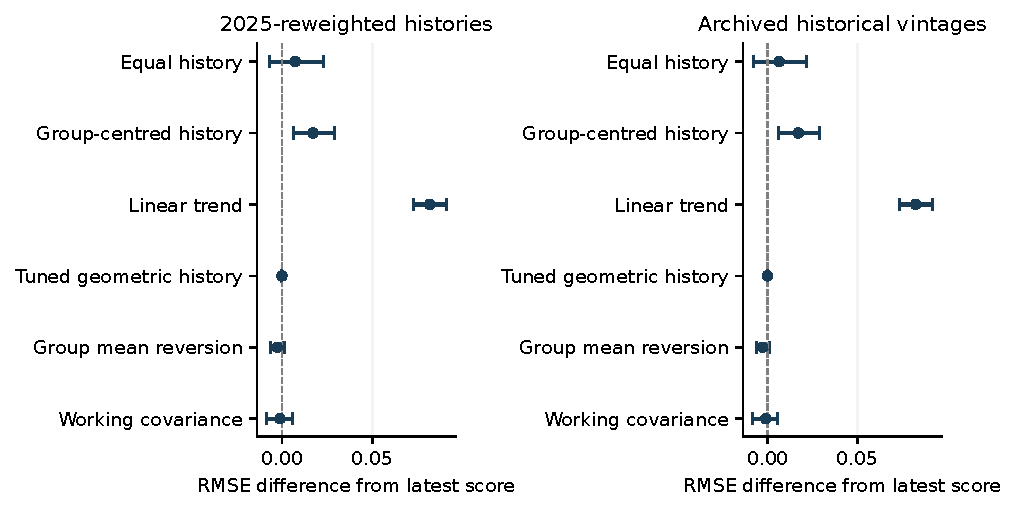
\includegraphics[width=\linewidth]{temporal_prediction.pdf}
\caption{Paired 95\% entity-bootstrap intervals for final RMSE differences. The harmonised and historical-vintage exercises use the same cohort and candidate grid. Small point gains for mean reversion and working covariance have intervals containing zero; linear extrapolation is markedly worse. These are conditional performance intervals, not intervals for intervention effects.}
\label{fig:prediction}
\end{figure}

Equal-history averaging is worse in point RMSE and MAE. Its RMSE difference interval includes zero, while its MAE difference interval is positive. Group-centred equal-history averaging and linear extrapolation perform worse more consistently in this test, with historical-vintage RMSEs 0.1472 and 0.2126, respectively. These results concern the declared four-year prediction rules and this cohort; they are not a theorem that historical information is harmful. The Gaussian projection result assumes a correct known model, whereas the empirical rules use estimated group centres and imperfect working structure.

The harmonised panel leads to the same broad conclusion (Appendix~\ref{app:empirical}). Its baseline RMSE is \RawHrmse{}, and the working-covariance rule's primary overlap is 61.1\%, one selected unit below the baseline. Historical reweighting slightly alters results, including membership near the cutoff, but does not overturn the substantive comparison. The additional archived-vintage analysis is necessary to make this finding rather than assume it.

\subsection{Selected low scores need not increase in the next year}
\begin{table}[t]
\centering\small\begin{tabular}{lrrrrr}
\toprule
Selection & Follow-up & Selected & $\Delta Y_S$ & $\Delta\mu_S$ & Difference \\
\midrule
2021 & 2022 & 36 & +0.0343 & +0.0184 & +0.0159 \\
2022 & 2023 & 36 & +0.2333 & +0.1803 & +0.0530 \\
2023 & 2024 & 36 & +0.0368 & +0.0074 & +0.0293 \\
2024 & 2025 & 36 & -0.0245 & -0.0635 & +0.0391 \\
\bottomrule
\end{tabular}

\caption{Observed follow-up of the within-group bottom-fraction rule in the harmonised panel. $\Delta\mu_S$ averages benchmark-group changes with weights induced by the selected units. The final column is $\Delta Y_S-\Delta\mu_S$; neither column is an estimated intervention effect.}
\label{tab:followup}
\end{table}

The 2024 selected group has an average score of 4.8279, falling to 4.8034 in 2025: a change of \SelectedChange{} points. Its corresponding benchmark-group change is \PeerChange{}, so it improves relative to those groups by \AdjustedChange{} points. Absolute deterioration and peer-relative improvement coexist. The positive relative difference is consistent with several mechanisms, including regression to the mean, differential shocks, intervention, response composition and model error. The data do not separate these mechanisms.

\begin{figure}[t]
\centering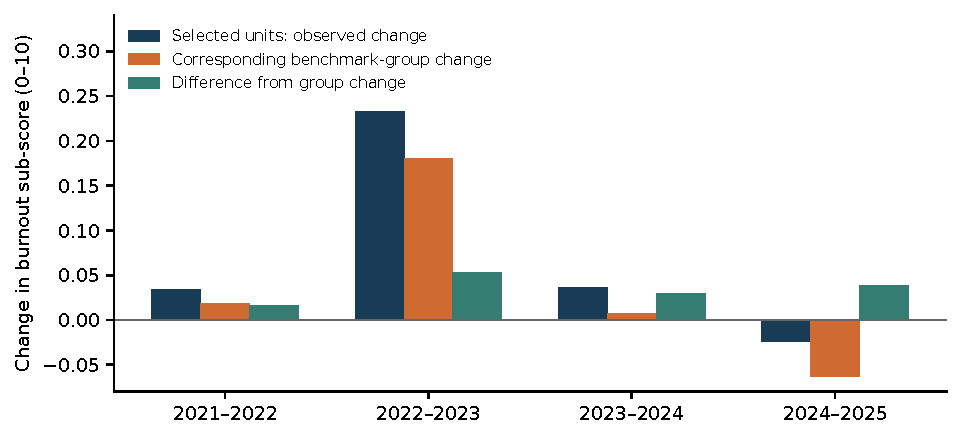
\includegraphics[width=.97\linewidth]{observed_followup.pdf}
\caption{Observed selected-group changes and contemporaneous benchmark-group changes. The 2022--2023 selected-group improvement mostly coincides with a wider group improvement. In 2024--2025, the selected group deteriorates in absolute terms while improving relative to its peers. No zero-intervention counterfactual is observed.}
\label{fig:followup}
\end{figure}

The 2022--2023 increase is much larger, approximately 0.2333 points, but about 0.1803 points coincide with the change in the corresponding benchmark groups. Ignoring that common movement would overstate how distinctive the selected units' trajectory is. Conversely, simply subtracting the group movement does not solve confounding or establish that the remaining 0.0530 points are attributable to wellbeing spending. Equation~\eqref{eq:causal_residual} applies to either a parametric or a peer-based reference prediction.

\subsection{The observed review list is fairly stable within the declared static model}
We apply~\eqref{eq:static_shrinkage} to 2025 deviations from the observed within-group means, using nominal valid burnout counts. The seven declared ratio values span $\lambda=0$ to $3000$; this range is a sensitivity specification, not a confidence region for the true ratio. We enumerate all pairwise crossings in the range and evaluate the intervening intervals.

\begin{table}[t]
\centering\small\begin{tabular}{lrrr}
\toprule
Benchmark group & $M$ & $k$ & First boundary $\lambda$ \\
\midrule
Acute specialist & 13 & 2 & None at finite $\lambda$ \\
Acute / acute-community & 110 & 22 & 234.60 \\
Ambulance & 11 & 2 & 11,990.84 \\
Community & 13 & 2 & 3,377.43 \\
Mental health / related & 43 & 8 & 24,822.36 \\
\bottomrule
\end{tabular}

\caption{First membership-changing boundary for the raw 2025 review set in each benchmark group. A large or absent boundary describes stability within the one-parameter working model. It is not a lower bound on the sample size required for reliable ranking. Values beyond 3000 lie outside the main plotted range.}
\label{tab:thresholds}
\end{table}

All 36 raw-selected units remain selected through the ratio grid up to 100. At 300, 35 remain; at 3000, 34 remain. Across the full breakpoint partition, the intersection contains 34 units and the union contains 38. The first membership change occurs in the acute/acute-community group at approximately $\lambda=234.60$. Other groups have no membership change within the declared range. Thus the organisation-level data do not support a claim that inverse-count adjustment radically reshuffles this particular review list.

\begin{figure}[t]
\centering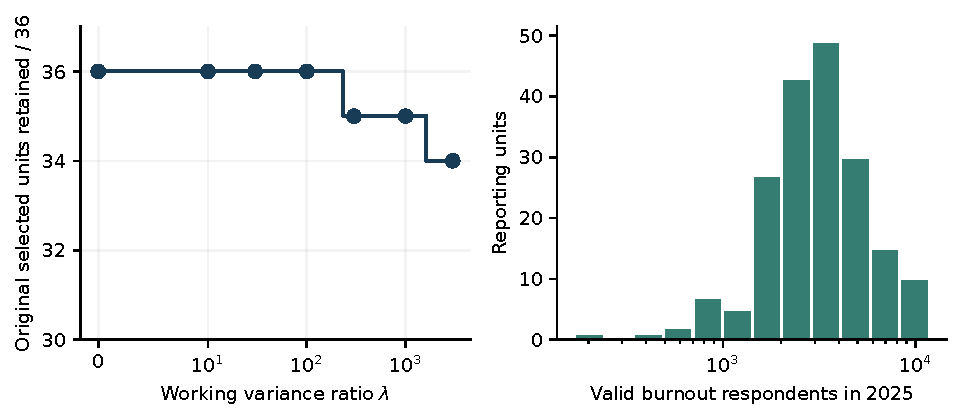
\includegraphics[width=\linewidth]{rank_sensitivity.pdf}
\caption{Static 2025 ranking sensitivity and observed response sizes. Left: retained members of the original 36-unit set, evaluated across analytical crossing intervals; markers show the declared ratio grid. Right: nominal valid burnout-response counts. Stability is conditional on fixed group centring and the common inverse-count noise-ratio model.}
\label{fig:sensitivity}
\end{figure}

This stability has a restricted interpretation. It does not establish that the common-ratio model is correct, that a stable response bias is absent, or that the chosen set maximises intervention benefit. In particular, Proposition~\ref{prop:nonid} permits observationally equivalent latent interpretations outside this sensitivity family. The result also cannot be transferred to departments containing only a few dozen respondents: the empirical cohort's smallest valid count is 170, and most units have substantially more.

\FloatBarrier
\section{Latent-truth simulations}
\subsection{Design and reproducibility}
Simulations use 80 independent units, five observed waves and one subsequent wave. The latent process has mean 5, standard deviation 0.35 and persistence $\phi\in\{0,0.3,0.6,0.85,0.97\}$. Nominal sizes are drawn once per design cell from a rounded log-uniform distribution over one of four ranges: 20--120, 40--250, 150--600 or 800--3000. They are held fixed across repetitions within the cell. Measurement variance is $\sigma^2/n_i$, with $\sigma^2\in\{1,6.25,25\}$ and error autocorrelation $\psi\in\{0,0.5\}$.

This produces 120 Gaussian design cells, each with 5,000 independent panel repetitions, or 600,000 independent simulated panels. Five rules and three selection fractions, $\{0.1,0.2,0.4\}$, are evaluated on the same panels. Those paired evaluations are not counted as additional independent experiments. Seed streams, per-cell counts, numerical summaries and Monte Carlo standard errors are saved.

The rules are the current score, an equal-history mean, a normalised geometric mean with the generating $\phi$, the Gaussian posterior using the correct covariance, and a posterior rule assuming white measurement error. The Gaussian rule has an oracle interpretation only in correctly specified cells; it is a working rule in misspecification stress tests. Means and trend paths are known to the simulation estimators. Latent severity regret and true-bottom-set overlap use the simulated current latent state, while rebound uses the actual next observed score. These quantities have different targets.

Gaussian observations are not clipped to the survey's 0--10 range, because clipping would change the exact conditional identities. Out-of-range frequencies are recorded. The simulations are stylised investigations of the model; their smaller size ranges are not observed NHS department data and their variance parameters are not estimates from the organisation panel.

\subsection{Pooling can trade noise for tracking error}
\begin{table}[t]
\centering\small\setlength{\tabcolsep}{3.5pt}
\begin{tabular}{lrrrrrr}
\toprule
Size range & Raw hit\% & Regret & Geom. hit\% & Regret & Gauss. hit\% & Regret \\
\midrule
20--120 & 55.6 & 0.1522 & 61.4 & 0.1124 & 64.4 & 0.0958 \\
40--250 & 63.7 & 0.1020 & 65.3 & 0.0899 & 70.3 & 0.0661 \\
150--600 & 77.4 & 0.0384 & 69.6 & 0.0687 & 79.8 & 0.0298 \\
800--3000 & 88.9 & 0.0084 & 71.3 & 0.0607 & 89.4 & 0.0077 \\
\bottomrule
\end{tabular}

\caption{Reference Gaussian simulation slice: $\phi=0.85$, $\sigma^2=6.25$, white measurement error and $k=16$ of 80 units. Hit is overlap with the realised latent bottom set; regret is the mean excess latent score per selected unit. These are assumed-parameter simulation results.}
\label{tab:simulation}
\end{table}

At the smallest size range, geometric history increases latent overlap from 55.6\% to 61.4\% and reduces average severity regret from 0.1522 to 0.1124. The correctly specified posterior yields overlap 64.4\% and regret 0.0958. At sizes 800--3000, geometric history instead reduces overlap from 88.9\% to 71.3\%, and increases regret from 0.0084 to 0.0607. The posterior remains close to the accurate current score, with regret 0.0077. These contrasting outcomes reflect fixed-weight tracking error and the advantage of a correctly specified conditional mean; they do not justify a universal count cutoff.

\begin{figure}[t]
\centering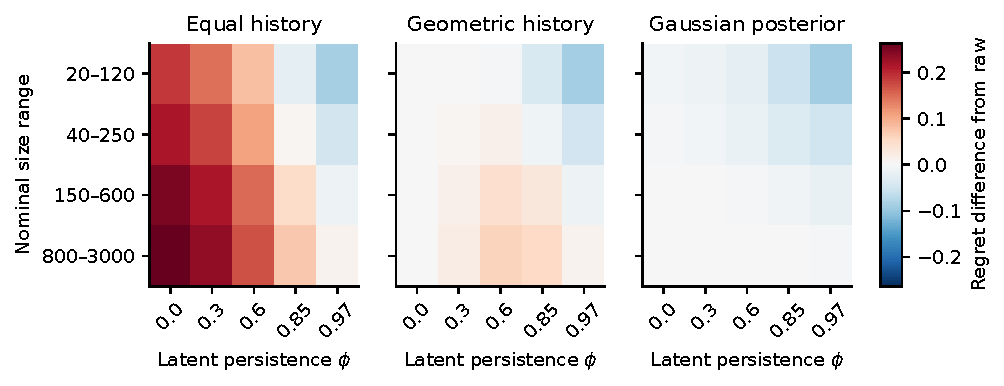
\includegraphics[width=\linewidth]{simulation_regret.pdf}
\caption{Average severity-regret difference from the current-score rule, for $\sigma^2=6.25$, $\psi=0$ and selection fraction 0.2. Blue denotes lower regret, red higher regret. Fixed historical weights can help or harm as persistence and precision change. The Gaussian posterior uses the true generating covariance in these cells.}
\label{fig:regret}
\end{figure}

The broad grid shows that sample size alone is an inadequate description of the tradeoff. When persistence is low, equal-history averaging can replace current information with obsolete states. Geometric history adapts partly through $\phi$, but remains a constrained normalised rule. The full posterior also shrinks toward the known mean and accounts for precision, which the fixed rules do not optimise. Its Bayes decision property concerns expected severity regret; Table~\ref{tab:simulation}'s overlap improvements in this slice do not establish overlap optimality in general.

\subsection{Conditional rebound agrees under the model and fails under misspecification}
For each selected set, we compare the simulated next-wave change with the conditional Gaussian prediction using all the information on which selection depends. Across the Gaussian grid, the mean residuals are consistent with Monte Carlo variation; the largest absolute residual divided by its Monte Carlo standard error is 3.48 across the many dependent method/fraction summaries. This is a numerical identity check, not a familywise significance test or empirical validation of a no-intervention model for NHS organisations.

\begin{figure}[t]
\centering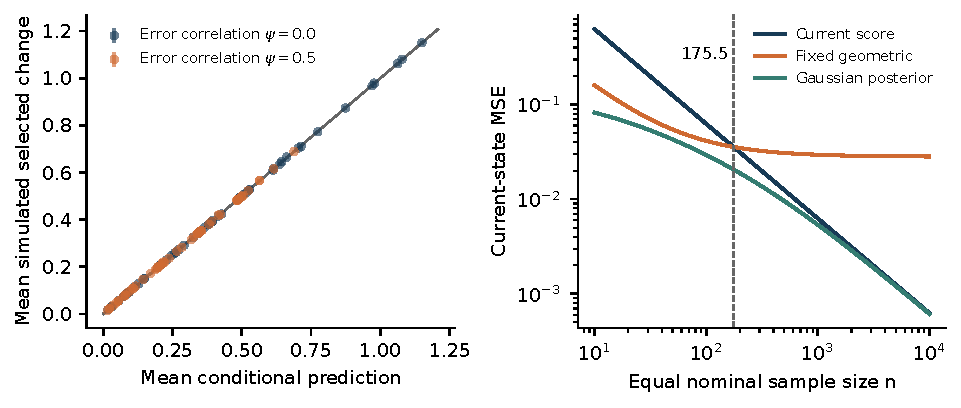
\includegraphics[width=\linewidth]{rebound_and_pooling.pdf}
\caption{Left: simulated versus conditional-predicted selected-group change for the raw bottom-20\% rule across 120 Gaussian cells. Error bars use 1.96 times the Monte Carlo standard error of the paired prediction residual. Right: exact current-state risks for equal $n$, five waves, $\phi=0.85$, $\tau=0.35$ and $\sigma=2.5$. The geometric crossover at 175.5 is conditional on these parameters and loss; the Gaussian posterior risk has no analogous penalty from adding correctly modelled history.}
\label{fig:identities}
\end{figure}

Prespecified stress tests replace Gaussian errors by variance-standardised Student-$t_3$ errors, impose a common annual decline, add a persistent unit-specific response bias, or increase measurement-error correlation to 0.9. A persistent bias with standard deviation 0.3 reduces raw latent overlap to 47.6\% in its small-unit scenario. Its mean selected rebound is 0.4111, while the Gaussian working prediction is 0.4876. The working posterior likewise overpredicts rebound. More data over time do not average away the persistent bias.

With measurement-error correlation 0.9, the correctly specified Gaussian rule has severity regret 0.1449 versus 0.1730 for the white-error posterior. Observed raw-score rebound is much smaller than in the corresponding white-error reference cells. The stress scenarios use separate random designs, so their numerical differences are descriptive scenario comparisons, not paired estimates of a single parameter's isolated causal effect. Appendix~\ref{app:stress} reports the complete stress slice and the interpretation of each rule.

\section{Implications, limitations and next evidence}
\paragraph{A useful review output.}
The available data support an auditable screen: state the within-group capacity rule, show the observed scores and valid-response counts, and identify which memberships depend on a declared noise assumption. For this cohort, most memberships remain stable over the specified static family. That can help focus additional investigation on a small number of boundary cases while preserving the distinction between a review list and a spending recommendation.

\paragraph{A better evaluation question.}
The selected group's next score should be reported alongside common trends and an explicitly conditional predictive reference. A manager evaluating a wellbeing programme needs a credible comparison design or additional assumptions about its untreated trajectory. A change exceeding a model mean is insufficient. Intervention assignments, timing, costs and outcomes would permit a new study; they cannot be reconstructed from a perceived-action item or from the present panel's forecast residuals.

\paragraph{What remains unidentified.}
The aggregate panel does not reveal individual weight distributions, composite-score variances, repeated respondent overlap or nonresponse bias. The restricted sensitivity family does not span all plausible errors. Good observed-score prediction and a stable working ranking therefore cannot certify latent need. A Bayesian statement would also have to propagate uncertainty about group centres, hyperparameters and model structure, rather than treating a fitted ratio as known truth.

\paragraph{Temporal and population limits.}
Only one final target year follows the 2024 development year, and both are retrospective. The historical-vintage analysis respects the retrieved predictor releases, but the cohort still uses future complete-history availability and may not generalise to newly formed or reorganised units. Known shared legal identity is handled in resampling; unrecorded system-level dependence remains. Group-specific samples are small, and the study is confined to England's NHS reporting system and this burnout measure.

\paragraph{Departmental validation.}
A genuine departmental study would require stable department identifiers, repeated comparable scores, valid response counts, appropriate design-based uncertainty and information about staffing and response composition. It would then need a held-out evaluation of the chosen decision objective. Neither the illustrative $n_{\rm crit}$ nor the nominal-size simulation ranges can be issued as validated operational thresholds for departments.

\paragraph{Conclusion.}
Worst-first selection links measurement, prediction and evaluation, but does not make them the same problem. Our theoretical diagnostics specify when particular claims follow; the versioned NHS application shows limited gains from temporal smoothing, substantial common movement in selected-group trajectories, and modest list changes within one static noise family. A defensible use of these results is transparent, assumption-sensitive review prioritisation followed by better measurement and an appropriate intervention evaluation.

\section*{Data, code and AI assistance}
The analysis uses public aggregate NHS releases and archived copies of official historical workbooks. Source manifests record URLs, capture or access times, file hashes, workbook cells, comparability decisions and missing precision fields. Reproducible programs produce the panel, simulations, forecasts, figures and tables. The code package contains derived research outputs and download instructions; it does not place downloaded third-party questionnaires or workbooks under a newly asserted permissive licence. No new staff questionnaire, individual-level data collection or intervention is conducted.

AI tools assisted with source discovery and checking, theory critique and derivation, study design, programming, execution and inspection of computations, and manuscript writing. Numerical findings come from executed code and saved results. The author is responsible for the claims, sources, code and interpretation, including validation of AI-assisted content. Automated and independent computational checks are documented without presenting them as completed human scientific review.

\FloatBarrier
\begingroup\small\raggedright
\interlinepenalty=10000
\setlength{\bibsep}{4pt}
\bibliographystyle{plainnat}
\bibliography{references}
\endgroup

\appendix
\section{Additional derivations and counterexamples}\label{app:proofs}
\subsection{Unconditional change of a finite \texorpdfstring{lowest-$k$}{lowest-k} set}
Assume the current units are iid with $Y_i\sim N(\mu,V)$, $V=\tau^2+R$, and future conditional coefficient $\beta=\phi\tau^2/V$. Let $Z_{(j)}$ denote the $j$th order statistic of $M$ independent standard normals and
\[
 c_{M,k}=-\frac1k\sum_{j=1}^k\E Z_{(j)}.
\]
For $1\le k<M$, symmetry and strict ordering imply $c_{M,k}>0$. Applying the conditional mean to the selected order statistics gives
\begin{equation}
 \E(\overline{\Delta Y}_S)=\Delta\mu+(1-\beta)\sqrt V\,c_{M,k}.
 \label{eq:unconditional}
\end{equation}
The constant can be calculated using
\[
 \E\left\{\frac1k\sum_{j=1}^k Z_{(j)}\right\}
 =\frac Mk\int_{-\infty}^{\infty}z\varphi(z)
    \Pr\{\operatorname{Bin}(M-1,\Phi(z))\le k-1\}\,dz.
\]
This is a finite-capacity expression. Selecting below a fixed population threshold $a$ instead yields $\varphi(a)/\Phi(a)$, which is not the exact finite-$M$ substitute for $c_{M,k}$. The formula also shows that an adverse common drift less than $-(1-\beta)\sqrt Vc_{M,k}$ reverses the expected rebound. In heteroscedastic settings, the conditional expression in Proposition~\ref{prop:rebound} remains the simpler exact calculation for an already observed selected set.

\subsection{Two-wave smoothing and degenerate cases}
For weights $(1-a,a)$ on current and previous centred scores, with independent errors of variances $R_t,R_{t-1}$,
\[
 \MSE(a)=R_t(1-a)^2+a^2\{R_{t-1}+2\tau^2(1-\phi)\}.
\]
The minimising weight is
\[
 a^*=\frac{R_t}{R_t+R_{t-1}+2\tau^2(1-\phi)}.
\]
A fixed $a>0$ improves on the current raw score exactly when
\[
 a<\frac{2R_t}{R_t+R_{t-1}+2\tau^2(1-\phi)}.
\]
If the latent process does not drift, the tracking penalty can vanish. If $w$ is simply the current-score selector, both $D(w)$ and $1-\|w\|^2$ vanish and no nontrivial crossover exists. These cases must not be handled by mechanically dividing by $D(w)$ in~\eqref{eq:n_threshold}. With correlated measurement errors, the cross term in $w^\top Rw$ must be retained.

\subsection{Gaussian conditioning with correlated measurement error}
For $T$ oldest-to-newest observations, write $C_\phi$ and $C_\psi$ for latent and error correlation matrices. With constant within-unit variance $R_i$,
\[
 \Sigma_i=\tau^2C_\phi+R_iC_\psi.
\]
The cross-covariance with the current latent state is the last row of $\tau^2C_\phi$, denoted $c_{i,0}^\top$. The cross-covariance with the next observed score is
\[
 c_{i,+}^\top=\phi c_{i,0}^\top+
               \psi R_i(C_\psi)_{T,\cdot}.
\]
Consequently the centred conditional current-state and next-observation means are $c_{i,0}^\top\Sigma_i^{-1}z_i$ and $c_{i,+}^\top\Sigma_i^{-1}z_i$. Their conditional variances are $\tau^2-c_{i,0}^\top\Sigma_i^{-1}c_{i,0}$ and $\tau^2+R_i-c_{i,+}^\top\Sigma_i^{-1}c_{i,+}$. These are the formulas used in the simulations. The future measurement term cannot be omitted when $\psi\ne0$.

\subsection{A conditional severity-regret bound}
Let $S_m$ select the $k$ smallest posterior means. On the event $|\theta_i-m_i|\le b_i$ for all $i$, optimality of $S_m$ implies
\[
 L_{\rm sev}(S_m,\theta)
 \le\frac1k\left\{\sum_{i\in S_m\setminus A_k}b_i+
                  \sum_{i\in A_k\setminus S_m}b_i\right\}.
\]
To prove this, add and subtract posterior means in the difference of selected sums and use $\sum_{S_m}m_i\le\sum_{A_k}m_i$. There are at most $2\min(k,M-k)$ terms. If the posterior marginals are Gaussian with standard deviations $s_i$, the choices
\[
 b_i=s_i\sqrt{2\log(2M/\delta)}
\]
give simultaneous posterior coverage at least $1-\delta$ by Gaussian tail bounds and a union bound. Posterior independence is unnecessary. This is a known-model posterior statement; it does not provide frequentist coverage for an unknown NHS variance model or account automatically for estimated hyperparameters.

\subsection{Exact membership probabilities in the illustrative example}
For independent continuous latent posteriors with densities $f_i$ and distribution functions $F_i$, the probability of being the single lowest unit is
\[
 p_i=\int f_i(x)\prod_{j\ne i}\{1-F_j(x)\}\,dx.
\]
Independent numerical quadrature produces the three probabilities reported after Proposition~\ref{prop:loss}; their sum is one up to integration error. Selecting by mean and by this probability optimises different expectations. The Gaussian posterior rule used in the large simulation grid targets severity, and is not relabelled as an overlap-optimal procedure.

\subsection{Static ranking paths and numerical ties}
For each pair, write $g_{ij}(\lambda)=a_{ij}+\lambda b_{ij}$. A nonzero $b_{ij}$ gives the candidate root $-a_{ij}/b_{ij}$. We retain roots in the sensitivity range, sort them, and evaluate one midpoint between each adjacent pair. The finite list of roots and interval memberships is reproducible from the published aggregate scores. At a root, either adjacent set may qualify as a lowest-$k$ set when a boundary pair ties. Floating-point evaluations can differ at machine precision exactly at a root; claims about unique membership apply to strict inequalities and open intervals. The implementation's deterministic ordering is a computational convention, not additional evidence of a strict scientific ordering.

\section{Additional empirical results}\label{app:empirical}
\begin{table}[htbp]
\centering\small\setlength{\tabcolsep}{4pt}
\begin{tabular}{lrrrr}
\toprule
Rule & RMSE & MAE & Overlap (\%) & $\Delta$RMSE 95\% interval \\
\midrule
Latest score & 0.1296 & 0.0935 & 63.9 & [+0.0000, +0.0000] \\
Equal history & 0.1370 & 0.1097 & 52.8 & [-0.0068, +0.0229] \\
Group-centred history & 0.1468 & 0.1080 & 52.8 & [+0.0063, +0.0289] \\
Linear trend & 0.2113 & 0.1772 & 63.9 & [+0.0727, +0.0909] \\
Tuned geometric history & 0.1296 & 0.0935 & 63.9 & [+0.0000, +0.0000] \\
Group mean reversion & 0.1270 & 0.0928 & 63.9 & [-0.0063, +0.0012] \\
Working covariance & 0.1286 & 0.0948 & 61.1 & [-0.0088, +0.0058] \\
\bottomrule
\end{tabular}

\caption{Harmonised 2025-reweighted historical-panel results. The meaning of metrics and entity-bootstrap intervals is the same as in Table~\ref{tab:vintage}.}
\end{table}
\begin{table}[htbp]
\centering\small\begin{tabular}{lrrr}
\toprule
Rule & $\phi$ & $\lambda$ & 2024 MSE \\
\midrule
Latest score & -- & -- & 0.01119 \\
Equal history & -- & -- & 0.02909 \\
Group-centred history & -- & -- & 0.01295 \\
Linear trend & -- & -- & 0.02343 \\
Tuned geometric history & 0.00 & -- & 0.01119 \\
Group mean reversion & 0.85 & -- & 0.01038 \\
Working covariance & 0.85 & 300 & 0.00950 \\
\bottomrule
\end{tabular}

\caption{Development-selected settings using historical vintages. The chosen geometric coefficient zero means that this tuned family selects the latest-score rule. The working ratio is a predictive hyperparameter, not an identified individual response variance.}
\end{table}

Within-group rounding gives two selected acute-specialist units, 22 acute/acute-community units, two ambulance units, two community units and eight mental-health/related units. The primary 36-unit target is therefore not exactly 20\% of 190. The released tables also give group-specific performance and selection fractions 0.1 and 0.3. The lowest-$k$ identity comparator in those tables is always the \emph{observed} 2025 score.

The point forecasts are equally weighted over reporting units. They do not weight an organisation with more employees as having greater budget importance. The entity bootstrap likewise preserves each resampled entity's observed reporting records and divides by their resulting number; it does not estimate staff-level sampling uncertainty. Keeping the linked Isle of Wight sectors together handles one documented dependency, rather than assuming a complete mapping of all NHS system relationships.

The selected tuning configurations are identical in the two data-vintage analyses. Their development losses differ because their historical scores and development targets differ. The 2023 archived workbook and 2024 archived workbook are independently hashed, rather than recreated by reversing 2025 reweighting. Original annual detailed spreadsheets are retained locally as provenance checks; the historical-vintage backtest specifically uses the multi-year benchmark files, not a silent splice of annual snapshots.

\section{Simulation stress results}\label{app:stress}
\begin{table}[htbp]
\centering\scriptsize\setlength{\tabcolsep}{3pt}
\begin{tabular}{llrrr}
\toprule
Stress & Rule & Latent regret & Observed change & Predicted change \\
\midrule
Heavy-tailed error & Current score & 0.1241 & +0.3755 & +0.4061 \\
Heavy-tailed error & Geometric history (known $\phi$) & 0.1098 & +0.1934 & +0.2039 \\
Heavy-tailed error & Gaussian posterior & 0.0903 & +0.2507 & +0.2652 \\
Heavy-tailed error & Assumed white error & 0.0903 & +0.2507 & +0.2652 \\
Common decline & Current score & 0.1527 & +0.1792 & +0.1795 \\
Common decline & Geometric history (known $\phi$) & 0.1134 & -0.0472 & -0.0463 \\
Common decline & Gaussian posterior & 0.0964 & +0.0229 & +0.0252 \\
Common decline & Assumed white error & 0.0964 & +0.0229 & +0.0252 \\
Persistent response bias & Current score & 0.2077 & +0.4111 & +0.4876 \\
Persistent response bias & Geometric history (known $\phi$) & 0.2022 & +0.1753 & +0.2756 \\
Persistent response bias & Gaussian posterior & 0.1854 & +0.2347 & +0.3301 \\
Persistent response bias & Assumed white error & 0.1854 & +0.2347 & +0.3301 \\
Strong error correlation & Current score & 0.1552 & +0.0880 & +0.0882 \\
Strong error correlation & Geometric history (known $\phi$) & 0.2017 & +0.0793 & +0.0787 \\
Strong error correlation & Gaussian posterior & 0.1449 & +0.0860 & +0.0865 \\
Strong error correlation & Assumed white error & 0.1730 & +0.0843 & +0.0835 \\
\bottomrule
\end{tabular}

\caption{Prespecified stress slice, $n$ in 20--120, $\phi=0.85$, $\sigma^2=6.25$ and selection fraction 0.2. Each stress has 5,000 independent panels. The Gaussian rule is correctly specified in the known-common-decline and strong-error-correlation cells, and a working rule under heavy tails or unmodelled persistent response bias. Trends are known to the simulation rules; these numbers do not demonstrate empirical trend estimation.}
\end{table}

The common-decline scenario reduces the mean by 0.25 points per year. Some history-selected sets have negative next-wave observed change even though the within-year ranking is unchanged by a common shift. In this particular raw-score small-unit scenario, measurement reversion remains large enough that its average change is positive. Equation~\eqref{eq:unconditional} supplies the general threshold for reversal.

The heavy-tailed scenario standardises Student-$t_3$ errors to unit variance before applying the measurement scale. Finite variance permits MSE comparisons, but the Gaussian conditional law is no longer exact. The persistent-bias scenario adds an independent time-constant unit effect with standard deviation 0.3 to observed responses while keeping the latent target unchanged. This is a synthetic representation of an unmodelled measurement component, not an estimate of NHS nonresponse bias. The final stress increases measurement-error persistence to 0.9 and shows the cost of treating it as white noise.

\section{Reproducibility and an evidence path for departmental use}\label{app:repro}
The package separates original downloads, derived data, analysis code and manuscript sources. Source manifests identify the official URLs, archived capture URLs, access times and hashes. The parser maps each retained numerical field to a workbook cell, and the independent validator compares the exported values to those cells. The complete-history cohort, exclusions and canonical benchmark groups are materialised as data rather than recomputed from name similarity.

The simulation script generates all 120 base cells and four stress cells from independent seed streams. A separate theory-check script verifies covariance calculations, varying-count predictions, pair-crossing intervals and the objective counterexample. It also reproduces the initial illustrative four-row simulation with its original assumed parameters, so its agreement is distinguishable from real-data validation. Numerical output files contain Monte Carlo standard errors and distributional quantiles; a 10th--90th percentile interval across simulated panel changes is not a confidence interval for their expected mean.

To reproduce the main study, retrieve and validate the official sources, build the harmonised and archived-vintage panels, execute the two empirical analyses and the latent-truth simulations, and regenerate the report figures and tables. The generated LaTeX sources compile independently of the raw workbooks. Computation dates remain the actual execution dates recorded in manifests.

A later departmental extension should begin with a new protocol and genuine departmental measurements. Stable department identifiers and changes in boundaries must be documented. Valid response counts, weighting and item covariance should support a variance estimator appropriate to that report. The target decision should specify whether it values low latent severity, set membership, an equity criterion or intervention benefit. A held-out panel can assess observed prediction, while latent validation needs additional measurement and intervention evaluation needs a comparison design. None of these steps is replaced by transferring the organisation-level score distribution to a smaller nominal count.

\end{document}
